\mychapter{Aplicação e Testes}
\label{Cap:aplicacaoTestes}

\section{Desenvolvimento do Sistema Supervisório}

O sistema supervisório é desenvlvido através de uma aplicação no Elipse SCADA. A finalidade desse sistema é a seguinte: através da comunicação Modbus, deve se feita com sucesso a leitura de dois sensores de temperatura, sendo um deles ligado ao módulo analógico do TPW-03 e o outro ao N2000 e demonstrar graficamente a variação dos valores descritos por eles quando submetidos à mudanças de temperatura. 

Tendo em vista o objetivo do sistema, cria-se em uma tela, dois objetos do tipo '\textit{Guage}' que irá indicar o valor de temperatura apontado pelos sensores, um '\textit{Trend Graph}' que plota a temperatura descrita nos sensores a cada 0.5 segundos e um '\textit{Bar Graph}' que torna mais clara a observação da diferença de temperatura que cada sensor está medindo em determinado instante de tempo. A interface desenvolvida é observada na Figura \ref{fig:Interface}.

\begin{figure}[h!]
\centering
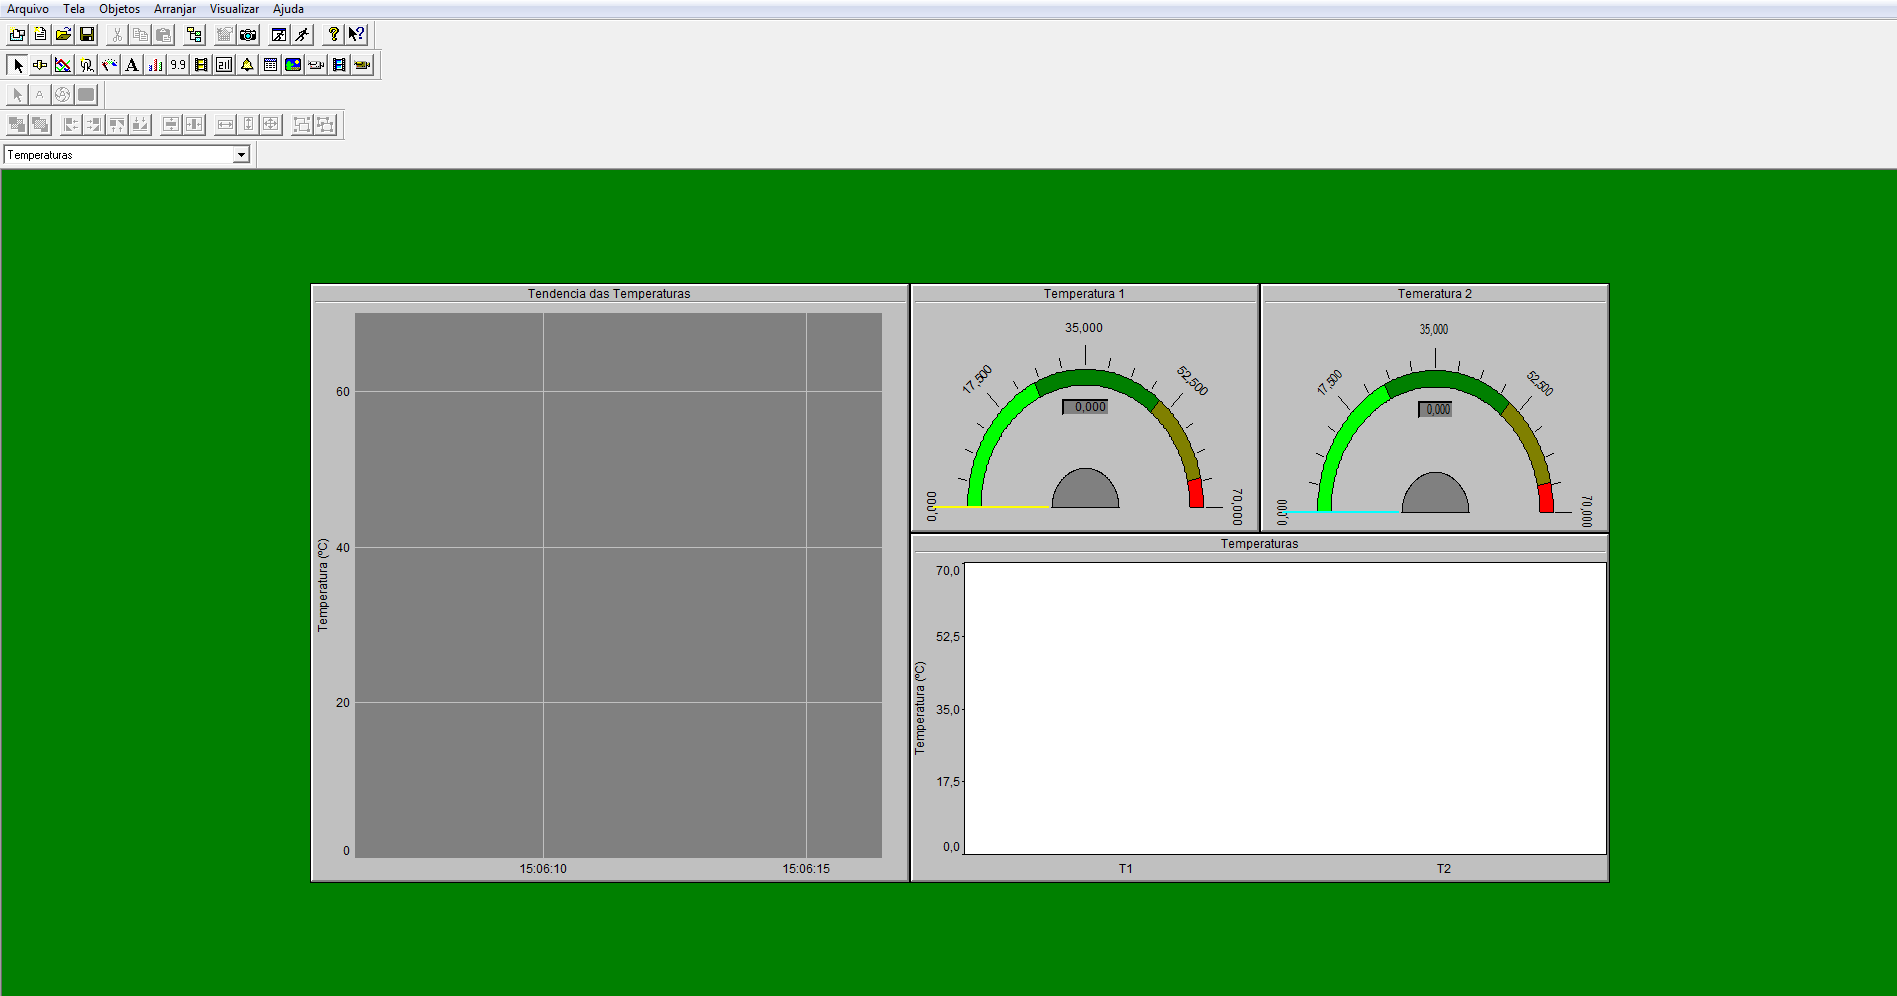
\includegraphics[scale=0.29]{Interface.png}
\caption{Interface da Aplicação}
\label{fig:Interface}
\end{figure}

Utilizando a ferramenta \textit{Organizer} do Elipse SCADA, criam-se duas \textit{tags} do tipo PLC, as quais irão armazenar as variáveis que indicam os valores das temperaturas fornecidas pelos sensores. Como essa aplicação consiste em um teste de conexão e leitura de apenas dois sensores, a utilização da \textit{tag} PLC atende aos requisitos do trabalho, visto que uma delas será associada ao TPW-03 (escravo 1) e a outra ao N2000 (escravo 2). Para sistemas maiores, com mais sensores a serem lidos, é mais conveniente a utilização da \textit{tag} Bloco PLC para os mesmos fins.

As \textit{tags} PLC e Bloco PLC funcionam de maneira similar, ambas são utilizadas para comunicação porém a primeira solicita apenas um endereço por consulta ao CLP, enquanto a segunda solicita vários endereços consecutivos em uma só chamada da função associada à tag.


A Figura \ref{fig:Organizer} demonstra a tela do \textit{Organizer} para a aplicação descrita. A fim de realizar a leitura dos sensores, deve-se configurar os parâmetros $N1$, $N2$, $N3$ e $N4$. Esses parâmetros são específicos de cada \textit{tag}. No caso da \textit{tag} PLC, temos os parâmetros:

\begin{itemize}
    \item $N1$: indica o endereço do equipamento (\textit{Slave Id}) para o TPW-03, primeiro escravo, configura-se $N1 = 1$.
    \item $N2$: indica o código da operação que será realizada. Nesse caso, deseja-se realizar uma leitura de um valor analógico, portanto deve-se escolher a operação que contenha uma função de leitura do tipo "\textit{3 - Read Holding Registers }" a operação de número $N2 = 4$ contém essa função (caso as operações padrões do \textit{driver} não tenham sido alteradas). Para observar, adicionar ou remover operações, deve-se verificar as configurações de operações do \textit{driver Modbus}.
    \item $N3$: parâmetro não utilizado pelo \textit{driver Modbus}, logo, $N3 = 0$.
    \item $N4$: indica o endereço do registro Modbus sobre o qual a \textit{tag} irá atuar, variando de acordo com a porta física onde o aparelho a ser lido está inserido.
\end{itemize}

O valor de N4 irá depender do endereçamento Modbus de cada equipamento. Para o TPW-03, o valor decimal utilizado (25644) observado na Figura \ref{fig:Organizer}, corresponde ao endereço de memória $D8436$ \cite{weg2010manualinstalacao}, o qual define o endereço Modbus da primeira entrada analógica do módulo de expansão 8AD (A0), onde o sensor de temperatura (correspondente à \textit{tag} $T1$) é ligado. 

Para o N2000, o valor de temperatura é armazenado na variável de processo (PV), correspondente ao endereço Modbus de número 0001 \cite{novus2014modbus}. Desse modo, o valor 0001 é estabelecido em $N4$ na\textit{tag} $T2$.

\begin{figure}[h!]
\centering
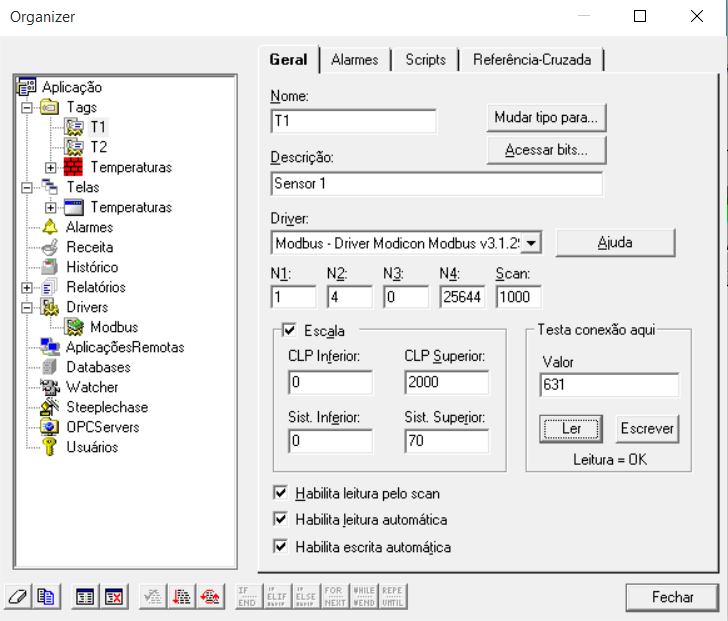
\includegraphics[scale=0.7]{Organizer.png}
\caption{\textit{Organizer} da aplicação}
\label{fig:Organizer}
\end{figure}

O valor definido na $Escala$ depende da resolução do sinal analógico gerado pelo CLP. No caso do TPW-03, utilizou-se o modo de entrada de corrente 4 - 20mA para conectar os sensores, o que nos dá uma resolução de 0 à 2000 unidades \cite{weg2010manualinstalacao}[p.65]. Dessa forma, configura-se a escala de 0 à 2000 unidades para o CLP indicando uma variação de temperatura proporcional de 0 a 70 ºC. Essa faixa de temperatura é estabelecida de acordo com os valores aos quais os transmissores dos sensores estão configurados.

A configuração do modo de operação do módulo 8AD é feita através da programação em Ladder no TPW03-PCLINK conforme explicado no item 3.2.1.


\section{Testes Desenvolvidos}

Feita a configuração de todos os parâmetros, associa-se as \textit{tags} a cada objeto criado através da própria tela da aplicação. Isso fará com que os objetos mostrem os valores lidos pelas \textit{tags} que representam as temperaturas dos sensores conectados aos controladores, logo, as medidas desejadas são mostradas nos elementos. Um exemplo da aplicação em atividade é observado na Figura \ref{fig:InterfaceRun}.

\begin{figure}[ht!]
\centering
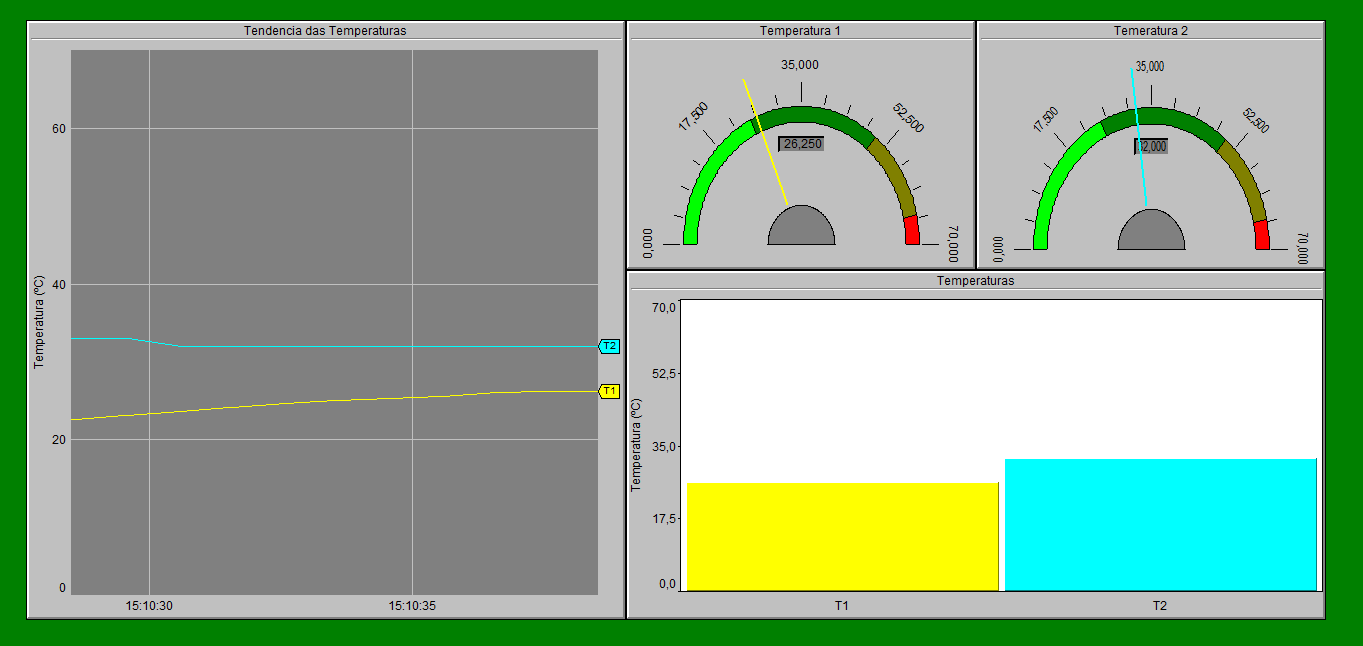
\includegraphics[scale=0.40]{InterfaceRun.png}
\caption{Aplicação em Execução}
\label{fig:InterfaceRun}
\end{figure}


Observa-se que os valores das temperaturas medidas nos dois sensores estão mostrados em todos os elementos da aplicação. Para testar o sistema, variou-se a temperatura nos dois sensores, conforme é observado no gráfico 'Tendência das Temperaturas'. O sensor que estava conectado ao TPW03 foi submetido à um aumento de temperatura simulado pelo contato dele a um corpo mais quente (temperatura de uma mão humana) enquanto o sensor conectado ao controlador N2000 foi submetido à uma diminuição de temperatura simulada por um copo de água gelada. As temperaturas obtidas durante o teste são coerentes, variando entre cerca de 20ºC e 35ºC.




%XXXXXXXXXXXXXXXXXXXXXXXXXXXXXXXXXXXXXXXXXXXXXXXXXXXXXXXXXXXXXXXXXXXXXXXXXXXXXXXXXXXXXXXXXXXXXXXXXXXXXXXX




